\documentclass{article}

\usepackage{fp}

\input{include/libs.tex}

\pgfmathsetmacro{\calwidth}{14}
\pgfmathsetmacro{\calheight}{22}

\newcommand{\calbox}{
    \draw [step=1,help lines] (0,0) grid (\calwidth,\calheight);
}

\newcommand{\calval}[3]{
    \node at (13-2*#1,2*#2+1) { \textbf{#3} };
}

\begin{document}
\begin{center}
    \pagestyle{empty}

    \vspace{1cm}
    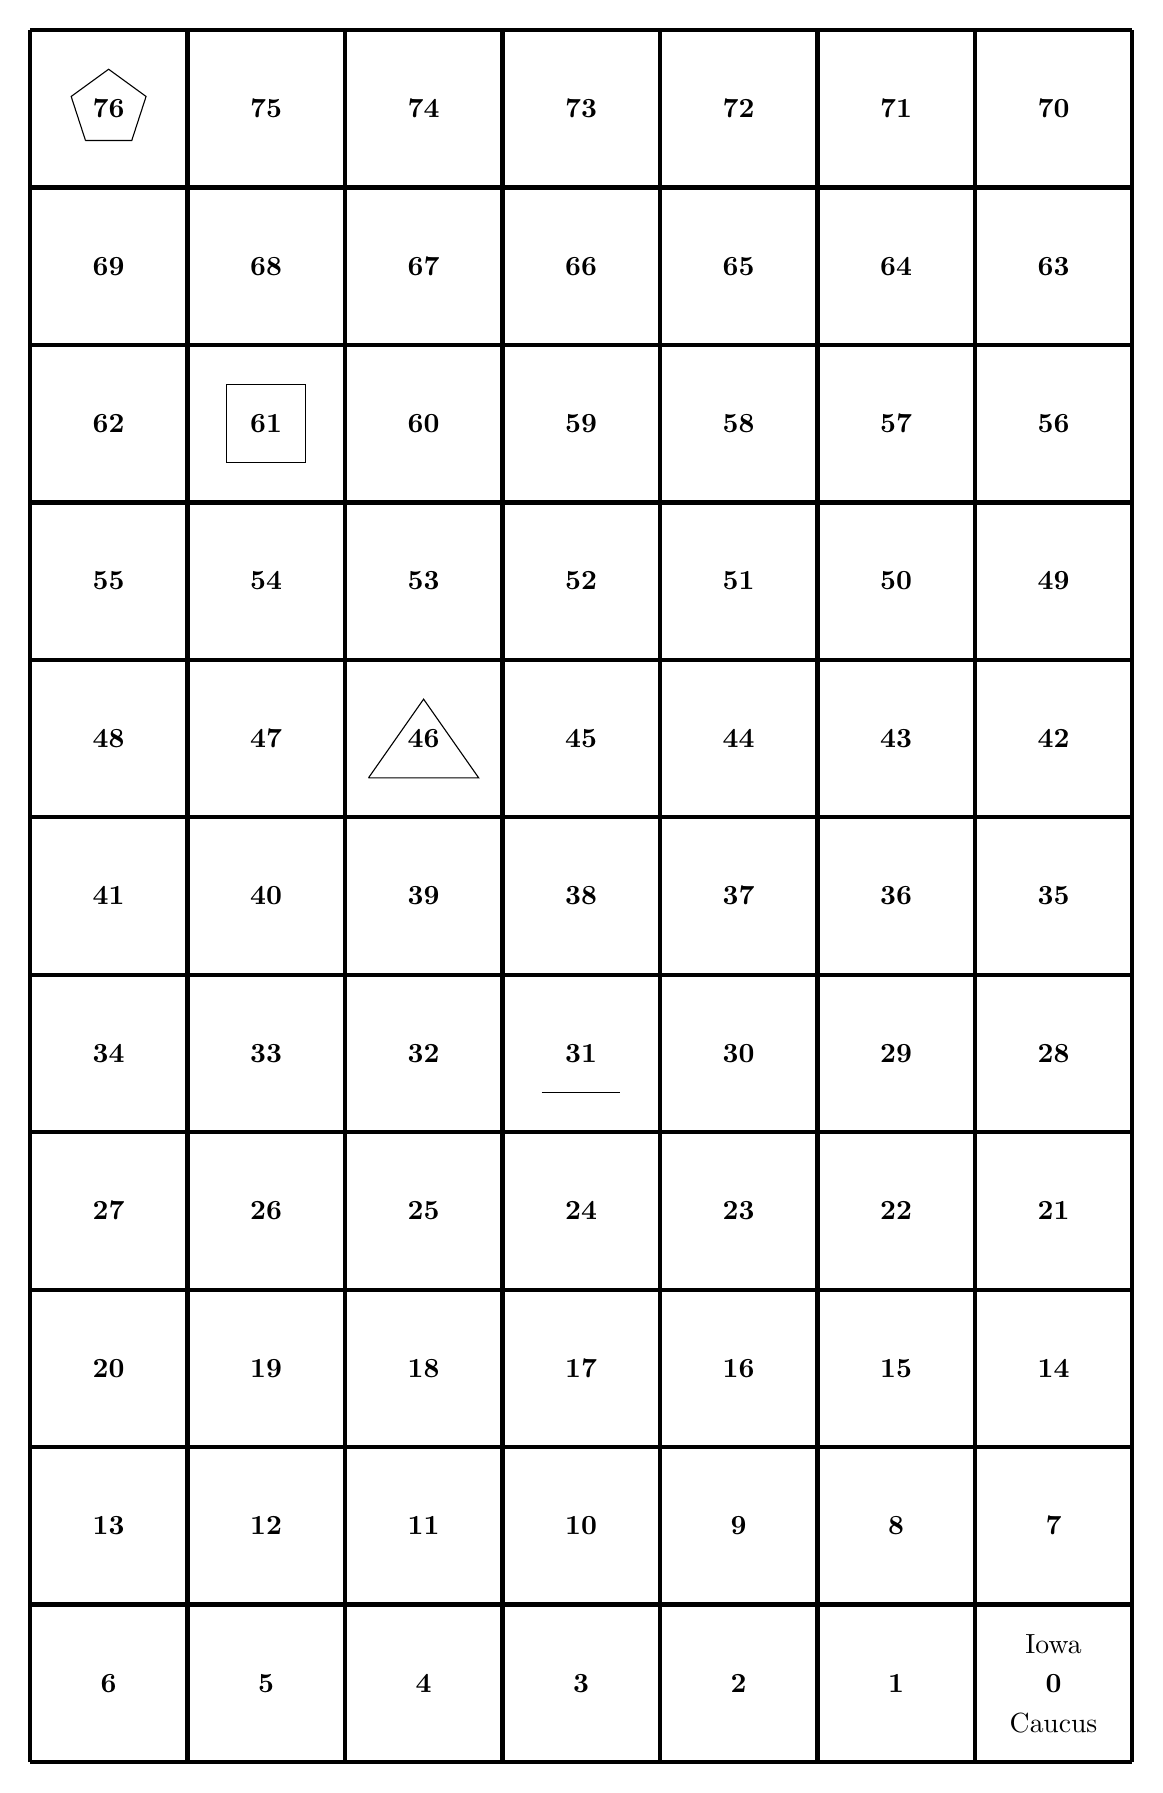
\begin{tikzpicture}
        %\calbox
        %\draw (0,0) rectangle(\calwidth,\calheight);
        \foreach \m in {7,...,0} {
            \draw [ultra thick] (2*\m,0) -- (2*\m,22);
        }
        \foreach \n in {0,...,11} {
            \draw [ultra thick] (0,2*\n) -- (14,2*\n);
        }
        \foreach \m in {0,...,6} {
            \foreach \k in {0,...,10} {
                \FPeval{\daynum}{round(\m+7*\k,0)}
                \calval{\m}{\k}{\daynum}
            }
        }

        \node at (13,1.5) {Iowa};
        \node at (13,0.5) {Caucus};

        % two player start line (square 31)
        \draw (6.5,8.5) -- (7.5,8.5);

        % three player start triangle (square 46)
        \draw (4.3,12.5) -- (5.7,12.5) -- (5,13.5) -- (4.3,12.5);

        % four player start square (square 61)
        \draw (2.5,16.5) -- (3.5,16.5) -- (3.5,17.5) -- (2.5,17.5) -- (2.5,16.5);

        % http://mathworld.wolfram.com/Pentagon.html
        % verticies calculated with pentagon perl script in this directory
        % five player start pentagon (square 76)
        \draw (0.7061,20.595) -- (1.2938,20.595) -- (1.4755,21.154) -- (1,21.5) -- (0.5244,21.154) -- (0.7061,20.595);
    \end{tikzpicture}

\vspace{1cm}
{\LARGE Calendar}

\end{center}
\end{document}
